% PREAMBLE
\documentclass[oneside,a4paper]{scrartcl}

% PACKAGES
%%%%%%%%%%
\usepackage[english]{babel}
\usepackage{graphicx}
\usepackage{pgf}
\usepackage{placeins}
\usepackage{listings}


% DOCUMENT
%%%%%%%%%%
%%%%%%%%%%

\begin{document}

%%%%%%%
% TITLE
%%%%%%%

\title{Exercise Sheet VIII}
\subject{Advanced Parallel Computing}
\author{Klaus Naumann \& Christoph Klein}
\maketitle

%%%%%%%
% PART 1 - Reading
%%%%%%%
\section*{Reading}
\subsection*{First Paper}
The paper 'The AMD Opteron Northbridge Architecture' from Pat Conway and Bill Hughes
published in 2007 presents an improved Northbridge architecture realized by AMD's
Direct Connect architecture, which uses an industry-standard HyperTransport technology
to link the processors with each other.

The main advantages of a HyperTransport interconnection are scalability, a high
bandwidth and wol latency. Furthermore the Direct Connect architecture provides
on chip integrated memory controller, thus reducing the front side bus bottlenecks.
The implemented HyperTransport protocol (HTP) ensures a coherent shared memory address
space. The HTP uses a broadcast-based coherence protocol, thus supports a good scaling
up to an eight-socket. Moreover this architecture has a lower power consumption
in comparison to the front side bus architecture.

To our mind this paper presents a detailed technical view on the new Northbridge
architecture, thus it provides useful information for the system architect, but not for
the system user. We would accept this paper, because sharing system architecture information
supports/accelerates system architecture developement.

\subsection*{Second Paper}
The paper 'The SGI Origin: a ccNUMA highly scalable server' from James Laudon and Daniel
Lenoski published in 1997 presents a chache-coherent non-uniform memory access (ccNUMA)
multiprocessor.

The caches are kept directory based coherent, which avoids
the broadcast bottleneck. The Origin symmetric multiprocessor architecture was designed
for dual-processor nodes with 4GB main memory and up to a maximum of 512 nodes.
As a network topology a bristled fat hypercube was choosen, where two nodes are
always connected to one SPIDER router. The used cache coherence protocol is alike
the DASH protocol, but has some improvements like the Clean-exclusive processor cache
state or full support of upgrade requests, without latency and bandwidth overhead
of moving the memory data. Furthermore the authors present the system performance using
the NAS Parallel benchmarks and the SPLASH2 suite.

To our mind this paper presents more a certain product rather than a new scientific
concept. Nevertheless we would acceppt this paper, because the system might be
well suited for certain scientific applications.


\section*{Red-Black Tree - Coarse-Grain Lock -- Development}
\label{dev}
We provide the code in different files, which we will explain shortly:
\begin{description}
    \item[./src/rbtreemain.c] This file contains our \texttt{main} function, the updatestream and 
				time-measurement functions and handles command line arguments. 
				You can choose the thread count, the search and insert operations.

\end{description}
The files \texttt{rbtree.c} and \texttt{rbtree.h} contain functions for several operations of the red-black
tree and were already provided in exercise 7.
As a lock we used \emph{pthread\_rwlock} which provides a shared read lock and an exclusive write lock.

\section*{Red-Black Tree - Coarse-Grain Lock -- Analysis}
We executed our program using various amount of threads and insert/search ratios. As you can see for each 
thread amount and ratio the executed operations per second are on a nearly constant level.  With increasing
insert operations the operations per second decrease. \\
 In figure \ref{plot_1090} the algorithm can execute between 1.00e+05 to nearly 3.00e+05 operations per second 
depending on the amount of threads. Here we used a ratio of 10/90 (insert/search). With a ratio of 90/10 (insert/search)
the possible operations per second decrease to a rate of 0.75e+05 to nearly 1.50e+05 as you can see in figure 
\ref{plot_9010}. The reason for this performance loss is the exclusive write-lock. At the time when one thread inserts a
node all other threads are spinning. 
    
\begin{figure}
	\centering
	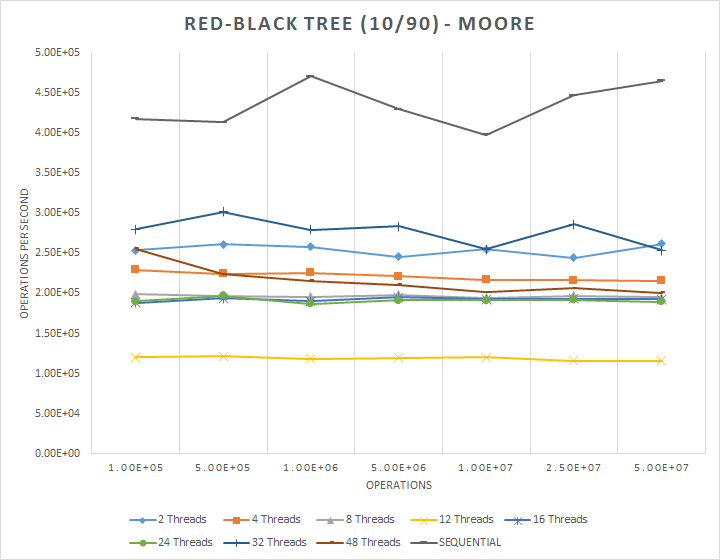
\includegraphics[width=1.0\textwidth]{results1090.png}
	\caption{Red-Black Tree test on \emph{moore} with a ratio of 10/90 (Insert/Search) for 1 to 48 threads.}
	\label{plot_1090}
\end{figure}

\begin{figure}
	\centering
	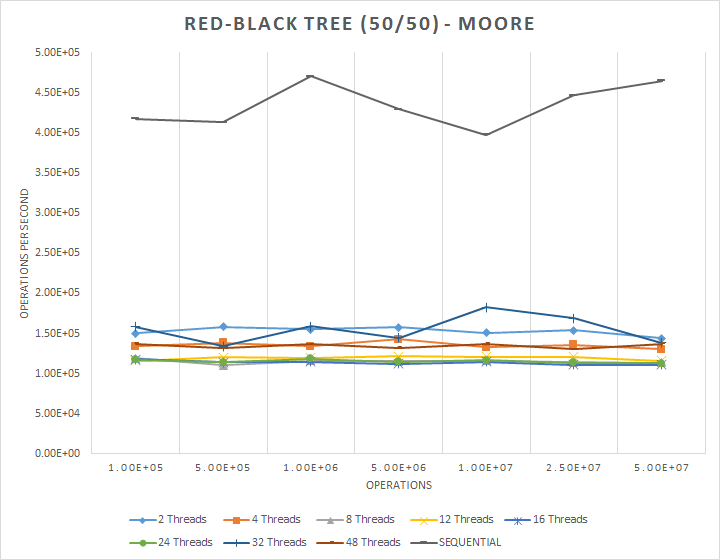
\includegraphics[width=1.0\textwidth]{results5050.png}
	\caption{Red-Black Tree test on \emph{moore} with a ratio of 50/50 (Insert/Search) for 1 to 48 threads.}
	\label{plot_5050}
\end{figure}

\begin{figure}
	\centering
	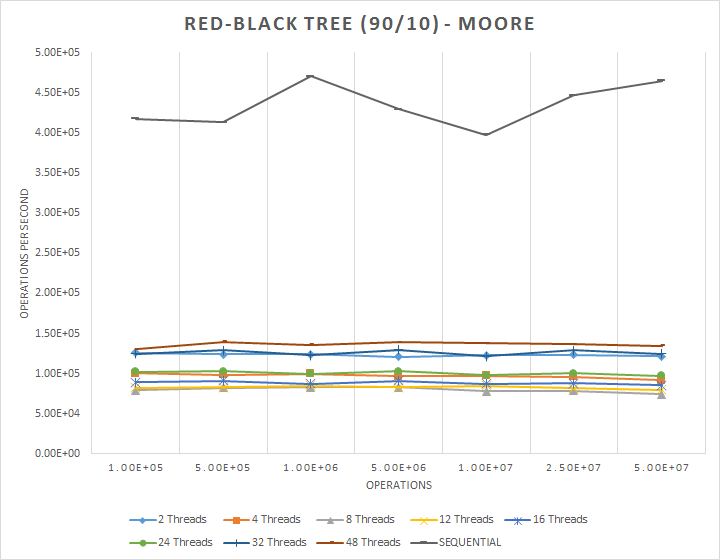
\includegraphics[width=1.0\textwidth]{results9010.png}
	\caption{Red-Black Tree test on \emph{moore} with a ratio of 90/10 (Insert/Search) for 1 to 48 threads.}
	\label{plot_9010}
\end{figure}
\end{document}
